\question
Kontrollstrukturen, wie z. B. Schleifen in höheren Programmiersprachen, werden in Maschinensprache über Sprungbefehle realisiert.
\begin{parts}
\part
Skizzieren Sie graphisch (schematisch), wie eine For- und eine While-Schleife, die 10-mal ($n \geq 0$) durchlaufen wird, umgesetzt werden könnte.
\begin{solutionordottedlines}[2cm]
1. For-Schleife
\begin{center}
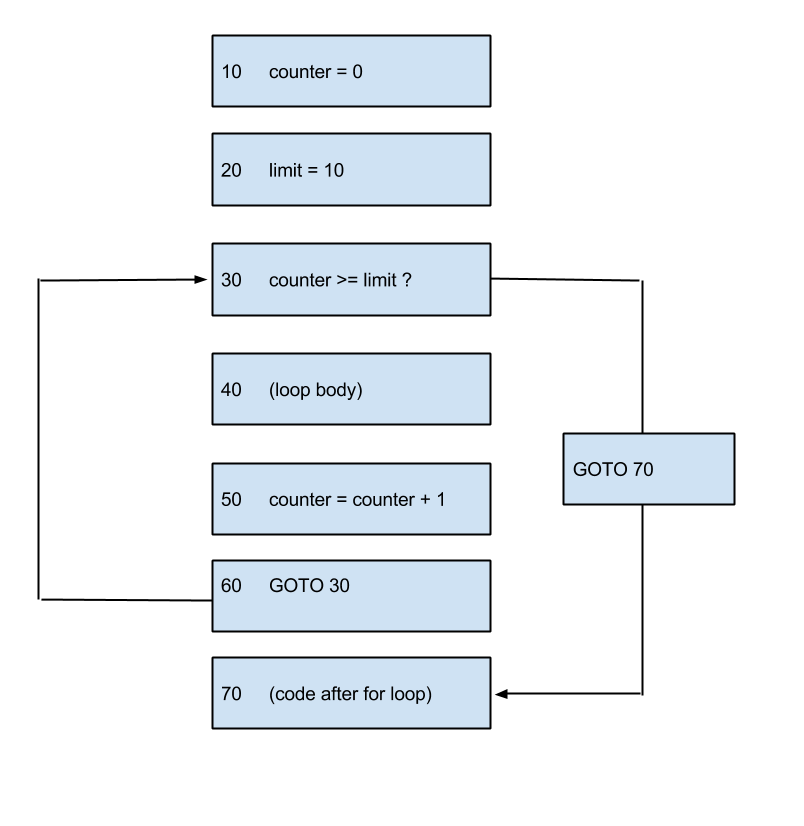
\includegraphics[width=\linewidth]{for-loop.png}
\end{center}
\pagebreak
2. While-Schleife
\begin{center}
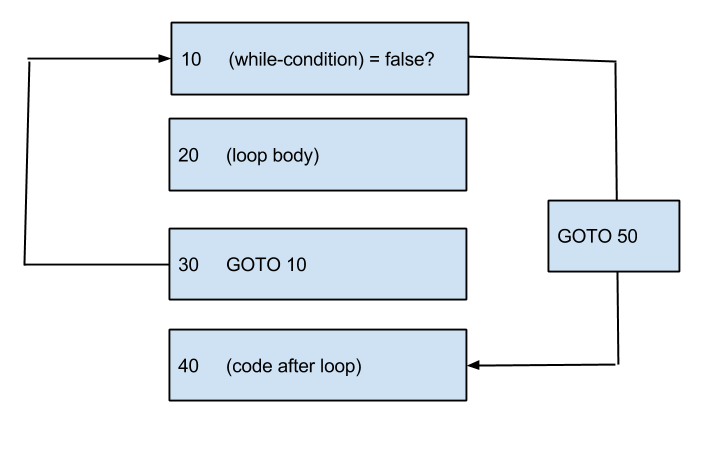
\includegraphics[width=\linewidth]{while-loop.png}
\end{center}
\end{solutionordottedlines}
%%% Next subquestion

\part
Mit welcher Einschränkung ist es möglich, die FOR-Schleife mit nur einem Sprungbefehl zu realisieren? Skizzieren Sie auch diesen Fall.
\begin{solutionordottedlines}[2cm]
\begin{center}
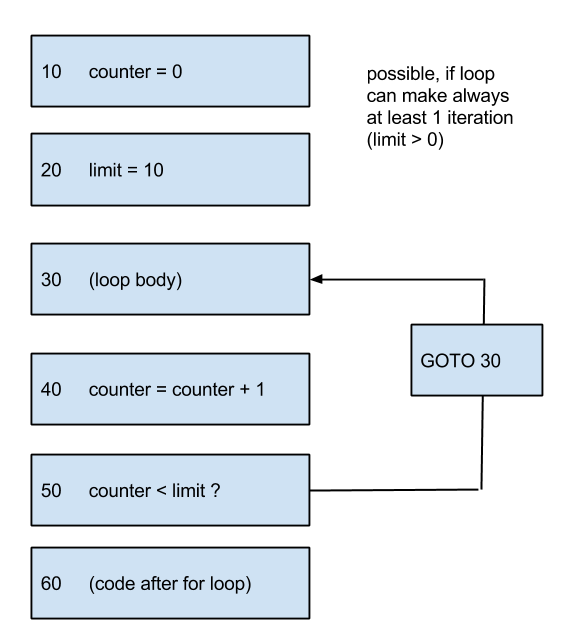
\includegraphics[width=0.7\linewidth]{for-loop-one-jump.png}
\end{center}
\end{solutionordottedlines}
%%% Next subquestion

\end{parts}